\section{A comparative evaluation of order-revealing encryption schemes and secure range-query protocols~\cite{ore-benchmark-17}}

	\begin{frame}{Survey of OPE/ORE schemes~\cite{ore-benchmark-17}}

		\begin{columns}[T,onlytextwidth]
			\column{0.5\textwidth}

				\begin{block}{The problem}

					\begin{itemize}
						\item Model: \alert{snapshot}, query type: \alert{range}
						\item Performance / security tradeoff
						\item Heterogeneous security definitions and leakage profiles
						\item \textbf{Performance of the schemes not well-understood}
						\begin{itemize}
							\item Some were not even implemented
							\item Prototype implementation at best
							\item Not benchmarked against one another
							\item Use different primitive implementations
						\end{itemize}
					\end{itemize}

				\end{block}

			\column{0.5\textwidth}

				\onslide<2->{
					\begin{block}{Our solution}

						\begin{itemize}
							\item Analyzed security and leakages of the constructions under a common framework
							\item Analyzed theoretically performance of the constructions
							\item \textbf{Implemented and run experiments}
							\begin{itemize}
								\item Implemented 5 OPE / ORE schemes and 5 range query protocols
								\item Used same language, framework and primitive implementations
								\item Benchmarked primitives execution times
								\item Counted primitives and I/O usage
							\end{itemize}
						\end{itemize}

					\end{block}
				}

		\end{columns}

	\end{frame}

	\begin{frame}{OPE / ORE schemes}

		\begin{adjustbox}{width=\linewidth}
			\begin{tabular}{ l c c c c c }

				\toprule

				\multirow{2}{*}{Scheme}						& \multicolumn{2}{c}{\onslide<2->{Primitive usage}}																						& \onslide<2->{Ciphertext size,}																& \onslide<2->{Leakage}																\onslide<2->{\\ \cline{2-3}}
				\rule{0pt}{10pt}							& \onslide<2->{Encryption}													& \onslide<2->{Comparison}									& \onslide<2->{or state size}																	& \onslide<2->{(In addition to inherent total order)}								\\

				\toprule

				BCLO~\cite{crypt-db-ope}					& \onslide<3->{$\bm{n}$ \textbf{HG}}										& \onslide<3->{none}										& \onslide<3->{$2n$}																			& \onslide<3->{\textbf{$\approx$ Top half of the bits}}								\\

				\midrule

				CLWW~\cite{practical-ore}					& \onslide<3->{$n$ PRF} 													& \onslide<3->{none}										& \onslide<3->{$2n$}																			& \onslide<3->{\textbf{Most-significant differing bit}}								\\

				\midrule

				\multirow{3}{*}{Lewi-Wu~\cite{lewi-ore}}	& \onslide<3->{\boldmath{} $\nicefrac{2n}{d}$ \unboldmath{} \textbf{PRP}}	& \onslide<3->{\multirow{3}{*}{$\frac{n}{2d}$ Hash}}		& \onslide<3->{\multirow{3}{*}{$\frac{n}{d} \left(\lambda + n + 2^{d + 1} \right) + \lambda$}}	& \onslide<3->{\multirow{3}{*}{Most-significant differing block}}					\\
															& \onslide<3->{$2 \frac{n}{d} \left( 2^d + 1 \right)$ PRF}					&															&																								&																					\\
															& \onslide<3->{$\frac{n}{d} 2^d$ Hash}										&															&																								&																					\\

				\midrule

				\multirow{3}{*}{CLOZ~\cite{adam-ore-v2}}	& \onslide<3->{$n$ PRF}														& \onslide<3->{\multirow{3}{*}{$\bm{n^2}$ \textbf{PPH}}}	& \onslide<3->{\multirow{3}{*}{$n \cdot h$}}													& \onslide<3->{\multirow{3}{*}{Equality pattern of most-significant differing bit}}	\\
															& \onslide<3->{$n$ PPH}														&															&																								&																					\\
															& \onslide<3->{1 PRP}														&															&																								&																					\\

				\midrule

				FH-OPE~\cite{fh-ope}						& \onslide<3->{1 Traversal}													& \onslide<3->{3 Traversals}								& \onslide<3->{$\bm{3 \cdot n \cdot N}$}														& \onslide<3->{Insertion order}														\\

				\bottomrule

			\end{tabular}
		\end{adjustbox}

	\end{frame}

	\begin{frame}{Range query protocols}

		\begin{adjustbox}{width=\linewidth}
			\begin{tabular}{ l c c c c c c }

				\toprule

				\multirow{2}{*}{Protocol}						& \multicolumn{2}{c}{\onslide<2->{{\IO} requests}}																																& \multirow{2}{*}{\onslide<2->{Leakage}}	& \multicolumn{2}{c}{\onslide<2->{Communication (result excluded)}}																&	\onslide<2->{\\ \cline{2-3} \cline{5-6}}
				\rule{0pt}{10pt}								& \onslide<2->{Construction}									& \onslide<2->{Query}																							&											& \onslide<2->{Construction}									& \onslide<2->{Query} 											&	\\

				\toprule

				{\BPlus} tree with ORE							& \onslide<3->{$\log_B \frac{N}{B}$}							& \onslide<3->{$\log_B \frac{N}{B} + \frac{r}{B}$}																& \onslide<3->{\textbf{Same as ORE}}		& \onslide<3->{$1$}												& \onslide<3->{$1$}												&	\\
				\midrule

				Kerschbaum~\cite{florian-protocol}				& \onslide<3->{$\bm{\frac{N}{B}}$}								& \onslide<3->{$\log_2 \frac{N}{B} + \frac{r}{B}$}																& \onslide<3->{\textbf{Total order}}		& \onslide<3->{$\log_2 N$}										& \onslide<3->{$\log_2 N$}										&	\\

				\midrule

				POPE~\cite{pope} warm							& \multirow{2}{*}{\onslide<3->{$1$}}							& \onslide<3->{$\log_L \frac{N}{B} + \frac{r}{B}$}																& \onslide<3->{\textbf{Partial order}}		& \multirow{2}{*}{\onslide<3->{$1$}}							& \onslide<3->{$\log_L N$}										&	\\

				POPE~\cite{pope} cold							& 																& \onslide<3->{$\bm{{\nicefrac{N}{B}}}$}																		& \onslide<3->{Fully hiding}				& 																& \onslide<3->{$\bm{N}$}										&	\\

				\midrule

				Logarithmic-BRC~\cite{practical-range-search}	& \onslide<3->{\textbf{---}}									& \onslide<3->{$\bm{r}$}																						& \onslide<3->{Same as SSE}					& \onslide<3->{\textbf{---}}									& \onslide<3->{$\log_2 N$}										&	\\

				\midrule

				\multirow{2}{*}{ORAM}							& \multirow{2}{*}{\onslide<3->{$\bm{{ \log^2 \frac{N}{B} }}$}}	& \multirow{2}{*}{\onslide<3->{$\bm{{ \log_2 \frac{N}{B} \left( \log_B \frac{N}{B} + \frac{r}{B} \right) }}$}}	& \onslide<3->{Fully hiding}				& \multirow{2}{*}{\onslide<3->{$\bm{{ \log^2 \frac{N}{B} }}$}}	& \multirow{2}{*}{\onslide<3->{$\bm{{ \log^2 \frac{N}{B} }}$}}	&	\\
																&																&																												& \onslide<3->{(access pattern)}			&																&																&	\\

				\bottomrule

			\end{tabular}
		\end{adjustbox}

	\end{frame}

	\begin{frame}{One of the experimental results}

		\begin{figure}[h]
			\centering
			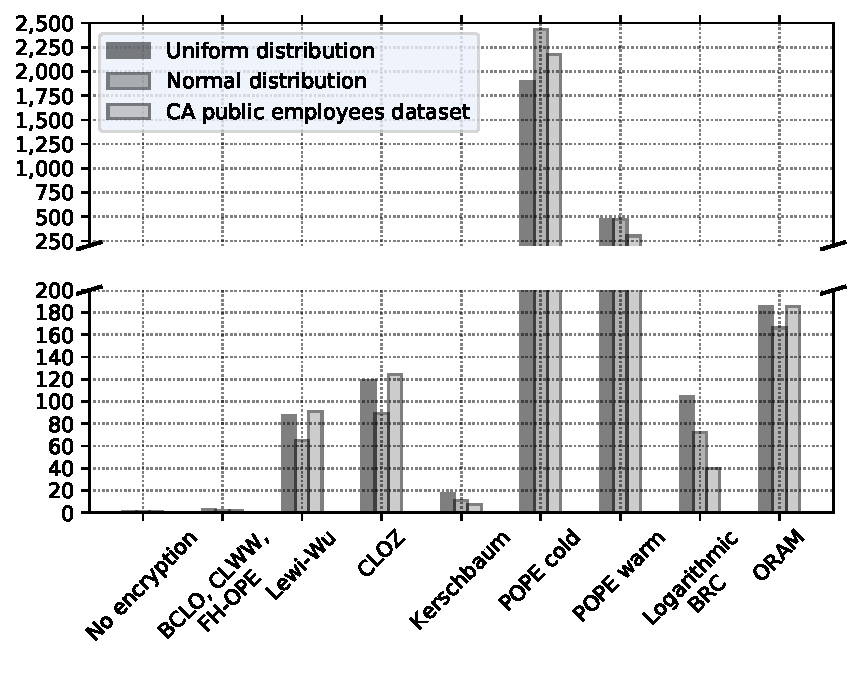
\includegraphics[width=0.6\textwidth]{protocol-charts-qios}
			\caption{Query stage number of I/O requests}
		\end{figure}

	\end{frame}
